\documentclass[11pt, a4paper]{article}
\usepackage[a4paper, margin=1in]{geometry}

\usepackage{adjustbox}
\usepackage{mathtools}
\usepackage{amsmath}
\usepackage{amssymb}
\usepackage{amsthm}

\usepackage{pgfplots}
\usepackage{listings}
\usepackage{color}
\usepackage{tikz}

\usepackage{textcomp}
\usepackage{soul}

\usepackage[hidelinks]{hyperref}
\pgfplotsset{width=7.5cm,compat=1.12}
\usepgfplotslibrary{fillbetween}
\pgfplotsset{compat=1.8}
\usepgfplotslibrary{statistics}
\usepackage[makeroom]{cancel}
\title{\bf{Homework \textnumero 13}}
\author{Author: David Oniani
\\
\ \ \ Instructor: Dr. Eric Westlund}
\date{April 5, 2019}

\usepackage{listings}
\usepackage{color}

%%%%%%%%%%%%%%% S E T S %%%%%%%%%%%%%%%
\newcommand{\nats}{\mathbb{N}}
\newcommand{\ints}{\mathbb{Z}}
\newcommand{\rats}{\mathbb{Q}}
\newcommand{\reals}{\mathbb{R}}
\newcommand{\irrats}{\mathbb{I}}

\newcommand{\pnats}{\mathbb{N}^+}
\newcommand{\pints}{\mathbb{Z}^+}
\newcommand{\prats}{\mathbb{Q}^+}
\newcommand{\preals}{\mathbb{R}^+}
\newcommand{\nreals}{\mathbb{R}^-}

\newcommand{\nints}{\mathbb{Z}^-}
\newcommand{\nrats}{\mathbb{Q}^-}
%%%%%%%%%%%%%%%%%%%%%%%%%%%%%%%%%%%%%%%

% Calligraphy
\newcommand\und[1]{\underline{\smash{#1}}}

% Operators
\DeclarePairedDelimiter\abs{\lvert}{\rvert}
\DeclarePairedDelimiter\ceil{\lceil}{\rceil}
\DeclarePairedDelimiter\floor{\lfloor}{\rfloor}

% Other
\newcommand{\rarr}{\rightarrow}

\definecolor{dkgreen}{rgb}{0,0.6,0}
\definecolor{gray}{rgb}{0.5,0.5,0.5}
\definecolor{mauve}{rgb}{0.58,0,0.82}
\definecolor{backcolour}{rgb}{0.95,0.95,0.92}

\lstset{
backgroundcolor=\color{backcolour},
aboveskip=3mm,
belowskip=3mm,
showstringspaces=false,
columns=flexible,
basicstyle={\small\ttfamily},
numbers=left,
numberstyle=\normalsize\color{gray},
keywordstyle=\color{blue},
commentstyle=\color{dkgreen},
stringstyle=\color{mauve},
breaklines=true,
breakatwhitespace=true,
tabsize=4
}


\begin{document}
\maketitle
\begin{itemize}
\item[18.2]
\begin{itemize}
\item[(a)]
From the Table A, we get that $z_{\alpha/2} = 1.96$.
Therefore, the confidence interval is from
\vspace{0.05cm}\\
$\overline{x} - 1.96 \times \dfrac{\sigma}{\sqrt{n}}$
to $\overline{x} + 1.96 \times \dfrac{\sigma}{\sqrt{n}}$ which is from 1.799 to 2.040.

\item[]

\item[(b)]
As the sample size is large (30 or more), the central limit theorem or CLT promises us
that the sampling distribution of the sample mean is approximately normal.

\item[]

\item[(c)]
The reasons are selection and non-response bias.\\
Selection bias as only the completed calls were present in the sample
and non-response bias bias as only 5029 calls from 45956 possible calls
were completed.
\end{itemize}

\item[]
\item[]

\item[18.6]
\begin{itemize}
\item[(a)]
Margin of Error = $1.96 \times \dfrac{7.5}{\sqrt{100}} = 1.47$.

\item[]

\item[(b)]
Margin of Error (400 young men) = $1.96 \times \dfrac{7.5}{\sqrt{400}} = 0.735$.
\vspace{0.05cm}\\
Margin of Error (1600 young women) = $1.96 \times \dfrac{7.5}{\sqrt{1600}} = 0.3675$.

\item[]

\item[(c)]
From the formula, it is easy to see that as sample size $n$ increases,
the Margin of Error decreases.
\end{itemize}

\item[]
\item[]

\item[18.8]
\begin{itemize}
\item[(a)]
\und{\textbf{State the hypothesis}}\\\\\\
$H_0: \mu = 514$ or $H_a: \mu > 514$
\\\\\\
\und{\textbf{Compute test statistic}}\\\\\\
$z = \dfrac{\overline{x} - \mu}{\dfrac{\sigma}{\sqrt{n}}} = \dfrac{541 - 514}{\dfrac{118}{\sqrt{50}}} \approx 1.62$
\\\\\\
\und{\textbf{Find the P-value}}\\\\\\
$P = P(z > 1.62) = P(z < -1.62) = 0.0526$
\\\\\\
\und{\textbf{State the conclusion}}\\\\\\
Since $P > \alpha$, the null hyopthesis is accepted
and the result is not statistically significant

\item[]

\item[(b)]
\und{\textbf{State the hypothesis}}\\\\\\
$H_0: \mu = 514$ or $H_a: \mu > 514$
\\\\\\
\und{\textbf{Compute test statistic}}\\\\\\
$z = \dfrac{\overline{x} - \mu}{\dfrac{\sigma}{\sqrt{n}}} = \dfrac{542 - 514}{\dfrac{118}{\sqrt{50}}} \approx 1.68$
\\\\\\
\und{\textbf{Find the P-value}}\\\\\\
$P = P(z > 1.68) = P(z < -1.68) = 0.0465$
\\\\\\
\und{\textbf{State the conclusion}}\\\\\\
Since $P < \alpha$, the null hyopthesis is rejected
and the result is statistically significant
\end{itemize}

\item[]
\item[]

\item[18.9]
\begin{itemize}
\item[(a)]
For $n = 9$, $z = \dfrac{4.8 - 5.0}{\dfrac{0.6}{\sqrt{9}}} = -1$ and $P = P(z < -1) = 0.1587$\\\\\\
For $n = 9$, $z = \dfrac{4.8 - 5.0}{\dfrac{0.6}{\sqrt{16}}} = -1.33$ and $P = P(z < -1.33) = 0.0918$\\\\\\
For $n = 9$, $z = \dfrac{4.8 - 5.0}{\dfrac{0.6}{\sqrt{36}}} = -2$ and $P = P(z < -2) = 0.0228$\\\\\\
For $n = 64$, $z = \dfrac{4.8 - 5.0}{\dfrac{0.6}{\sqrt{36}}} = -2.67$ and $P = P(z < -2.67) = 0.0038$\\\\
And obviously, we observe that as the sample size increases,
the $P$-value decreases.
\item[]

\item[(b)]
For $n = 9$
\begin{center}
    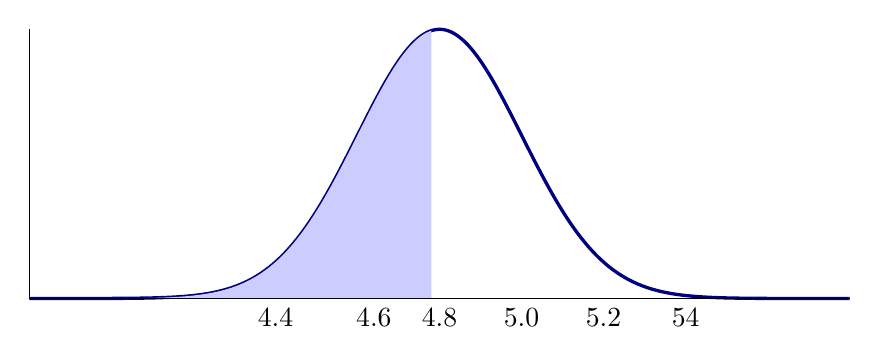
\begin{tikzpicture}
        \pgfmathdeclarefunction{gauss}{2}{%
        \pgfmathparse{1/(#2*sqrt(2*pi))*exp(-((x-#1)^2)/(2*#2^2))}%
        }
        \begin{axis}[
          no markers, domain=-5:5, samples=1000,
          axis lines*=left,
          height=5cm, width=12cm,
          xtick=\empty, ytick=\empty,
          enlargelimits=false, clip=false, axis on top,
          grid = major
          ]
          \addplot [very thick, blue!50!black] {gauss(0,1)};
          \addplot [fill=blue!20, draw=none, domain=-5:-0.1] {gauss(0,1)} \closedcycle;
          \node [below] at (300, 0) {$4.4$};
          \node [below] at (420, 0) {$4.6$};
          \node [below] at (500, 0) {$4.8$};
          \node [below] at (600, 0) {$5.0$};
          \node [below] at (700, 0) {$5.2$};
          \node [below] at (800, 0) {$54$};
        \end{axis}
    \end{tikzpicture}
    \end{center}

\item[]
\item[]

For $n = 16$
\begin{center}
    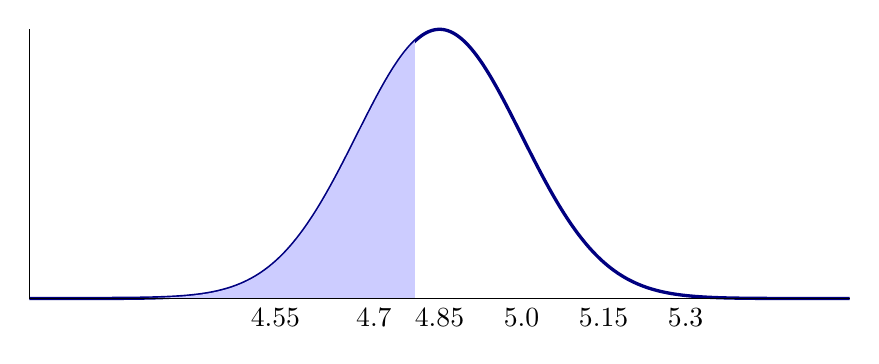
\begin{tikzpicture}
        \pgfmathdeclarefunction{gauss}{2}{%
        \pgfmathparse{1/(#2*sqrt(2*pi))*exp(-((x-#1)^2)/(2*#2^2))}%
        }
        \begin{axis}[
          no markers, domain=-5:5, samples=1000,
          axis lines*=left,
          height=5cm, width=12cm,
          xtick=\empty, ytick=\empty,
          enlargelimits=false, clip=false, axis on top,
          grid = major
          ]
          \addplot [very thick, blue!50!black] {gauss(0,1)};
          \addplot [fill=blue!20, draw=none, domain=-5:-0.3] {gauss(0,1)} \closedcycle;
          \node [below] at (300, 0) {$4.55$};
          \node [below] at (420, 0) {$4.7$};
          \node [below] at (500, 0) {$4.85$};
          \node [below] at (600, 0) {$5.0$};
          \node [below] at (700, 0) {$5.15$};
          \node [below] at (800, 0) {$5.3$};
        \end{axis}
    \end{tikzpicture}
    \end{center}

For $n = 36$
\begin{center}
    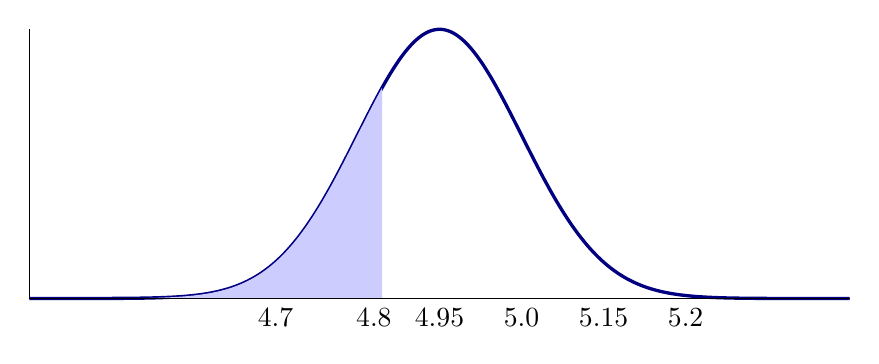
\begin{tikzpicture}
        \pgfmathdeclarefunction{gauss}{2}{%
        \pgfmathparse{1/(#2*sqrt(2*pi))*exp(-((x-#1)^2)/(2*#2^2))}%
        }
        \begin{axis}[
          no markers, domain=-5:5, samples=1000,
          axis lines*=left,
          height=5cm, width=12cm,
          xtick=\empty, ytick=\empty,
          enlargelimits=false, clip=false, axis on top,
          grid = major
          ]
          \addplot [very thick, blue!50!black] {gauss(0,1)};
          \addplot [fill=blue!20, draw=none, domain=-5:-0.7] {gauss(0,1)} \closedcycle;
          \node [below] at (300, 0) {$4.7$};
          \node [below] at (420, 0) {$4.8$};
          \node [below] at (500, 0) {$4.95$};
          \node [below] at (600, 0) {$5.0$};
          \node [below] at (700, 0) {$5.15$};
          \node [below] at (800, 0) {$5.2$};
        \end{axis}
    \end{tikzpicture}
    \end{center}

For $n = 64$
\begin{center}
    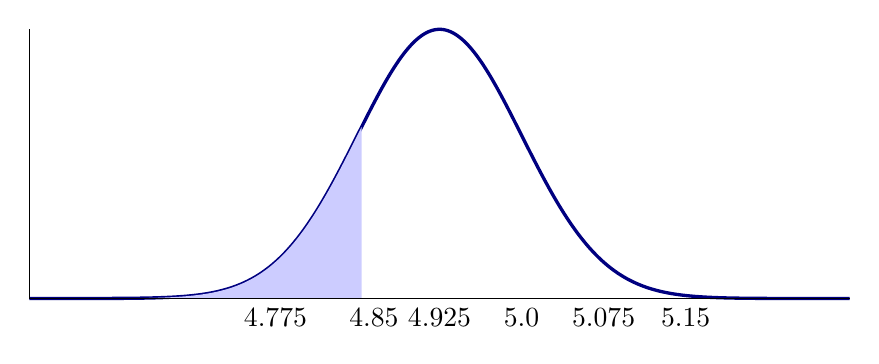
\begin{tikzpicture}
        \pgfmathdeclarefunction{gauss}{2}{%
        \pgfmathparse{1/(#2*sqrt(2*pi))*exp(-((x-#1)^2)/(2*#2^2))}%
        }
        \begin{axis}[
          no markers, domain=-5:5, samples=1000,
          axis lines*=left,
          height=5cm, width=12cm,
          xtick=\empty, ytick=\empty,
          enlargelimits=false, clip=false, axis on top,
          grid = major
          ]
          \addplot [very thick, blue!50!black] {gauss(0,1)};
          \addplot [fill=blue!20, draw=none, domain=-5:-0.95] {gauss(0,1)} \closedcycle;
          \node [below] at (300, 0) {$4.775$};
          \node [below] at (420, 0) {$4.85$};
          \node [below] at (500, 0) {$4.925$};
          \node [below] at (600, 0) {$5.0$};
          \node [below] at (700, 0) {$5.075$};
          \node [below] at (800, 0) {$5.15$};
        \end{axis}
    \end{tikzpicture}
    \end{center}
\end{itemize}

\item[]
\item[]

\item[18.10]
The confidence interval is from $4.8 - 1.96 \times \dfrac{0.6}{\sqrt{n}}$
to $4.8 + 1.96 \times \dfrac{0.6}{\sqrt{n}}$.\\\\
Thus, we have:\\\\
For n = 9, we have the confidence interval from 4.408 to 5.192.\\
For n = 16, we have the confidence interval from 4.506 to 5.094.\\
For n = 16, we have the confidence interval from 4.604 to 4.996.\\
For n = 16, we have the confidence interval from 4.653 to 4.947.

\item[]
\item[]

\item[18.12]
Let's use the formula for the sample size which is
$n = \Big(\dfrac{z_{\alpha/2} \times \sigma}{E}\Big)^2$.\\\\
We get that $n = \Big(\dfrac{1.96 \times 7.5}{1}\Big)^2 \approx 217$.

\item[]
\item[]

\item[18.13]
Let's use the formula for the sample size which is
$n = \Big(\dfrac{z_{\alpha/2} \times \sigma}{E}\Big)^2$.\\\\
We get that $n = \Big(\dfrac{1.645 \times 125}{10}\Big)^2 \approx 423$.

\item[]
\item[]

\item[18.33]
The effect of the outlier is obviously greater when the sample size
is small. With large sample sizes, the effect of the outlier is relatively low.

\item[]
\item[]

\item[18.36]
\begin{itemize}
\item[(a)]
Test of significance does not answer this question.
The researchers determine whether the design is proper or not.

\item[]

\item[(b)]
Test of significance answers this question.
A significance test takes into consideration the sampling error, which is indeed the observed effect due to chance.

\item[]

\item[(c)]
Test of significance does not answer this question.
The researchers determine whether the observed effect is important or not.
\end{itemize}

\end{itemize}

\end{document}
